%Berechnet mit https://tools.timodenk.com/cubic-spline-interpolation

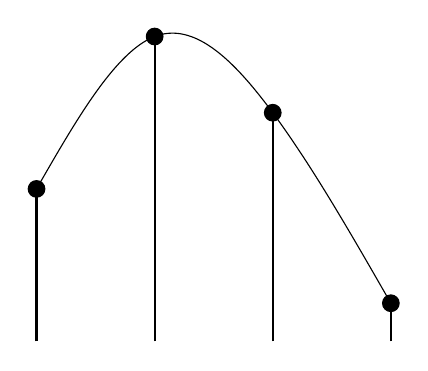
\begin{tikzpicture}[scale = 1.5]
    
        \pgfmathsetmacro\rEins{(+-0.7*0^3+1.32e-62*0^2+2.7*0^1+2*0^0)/1.55}
        \draw[thick, black, -](0,0) -- (0,\rEins);
        \draw[fill = black](0,\rEins) circle (2pt);

        \pgfmathsetmacro\rZwei{(+-0.7*1^3+1.32e-62*1^2+2.7*1^1+2*1^0)/1.55}
        \draw[thick, black, -](1,0) -- (1,\rZwei);
        \draw[fill = black](1,\rZwei) circle (2pt);

        \pgfmathsetmacro\rDrei{(+0.5*2^3+-3.6*2^2+6.3*2^1+0.8*2^0)/1.55}
        \draw[thick, black, -](2,0) -- (2,\rDrei);
        \draw[fill = black](2,\rDrei) circle (2pt);

        \pgfmathsetmacro\rVier{(+0.2*3^3+-1.8*3^2+2.7*3^1+3.2*3^0)/1.55}
        \draw[thick, black, -](3,0) -- (3,\rVier);
        \draw[fill = black](3,\rVier) circle (2pt);


    \draw[domain=0:1, smooth, variable=\x, black] plot ({\x}, {(+-0.7*\x^3+1.32e-62*\x^2+2.7*\x^1+2*\x^0)/1.55});
    \draw[domain=1:2, smooth, variable=\x, black] plot ({\x}, {(+0.5*\x^3+-3.6*\x^2+6.3*\x^1+0.8*\x^0)/1.55});
    \draw[domain=2:3, smooth, variable=\x, black] plot ({\x}, {(+0.2*\x^3+-1.8*\x^2+2.7*\x^1+3.2*\x^0)/1.55});
\end{tikzpicture}